\chapter{Turbostratic carbons II: Impregnation methods}
\label{ch:impregnation}

\newpage

\section{Introduction}

\section{Synthesis}
The author investigated additional precursors with high amounts of cellulosic material, therein using small amounts of porogen, and mixing the precursor and porogen in such a manner as to both minimise the distance between porogen and precursor, and evenly distribute the porogen. Firstly, sawdust-derived carbons were made by incorporating KOH at weight ratios between 0.00 and 2.00 into the hydrothermal carbonisation step, drying the resultant slurry overnight at $\rm 100\  ^{\circ}C$ and then activating at $\rm 800\ ^{\circ}C$ as usual. Hydrothermal carbonisation occured at 200, 250 or 300 $\rm ^{\circ}C$. These sawdust-derived hydrochars are designated \textit{SAx.xx-HHH} where the prefix \textit{SA} indicates activated sawdust, \textit{x.xx} is the KOH:sawdust ratio and \textit{HHH} is the hydrothermal carbonisation temperature. All samples were washed in the normal manner following activation. The hydrothermally carbonised intermediates are referred to as \textit{SHx.xx-HHH} to differentiate from the activated samples.
% should the lower TTT samples be included?

Additionally, sodium carboxymethyl cellulose (see figure \ref{fig:nc_structure}) was used as a precursor for direct (without hydrothermal carbonisation) activation. The porogen in this case is the sodium carboxymethyl group, and the porogen:precursor ratio is controlled by the degree of substitution. Samples are designated as \textit{NCx.x-TTT} where \textit{NC} indicates sodium carboxymethyl cellulose, \textit{x.x} is the degree of substitution, and \textit{TTT} is the activation temperature. Values for \textit{x.x} were 0.0, 0.7, 0.9, and 1.2 and \textit{TTT} was 600, 700, or 800 $\rm ^{\circ}C$.

\begin{figure}[h]
    \centering
    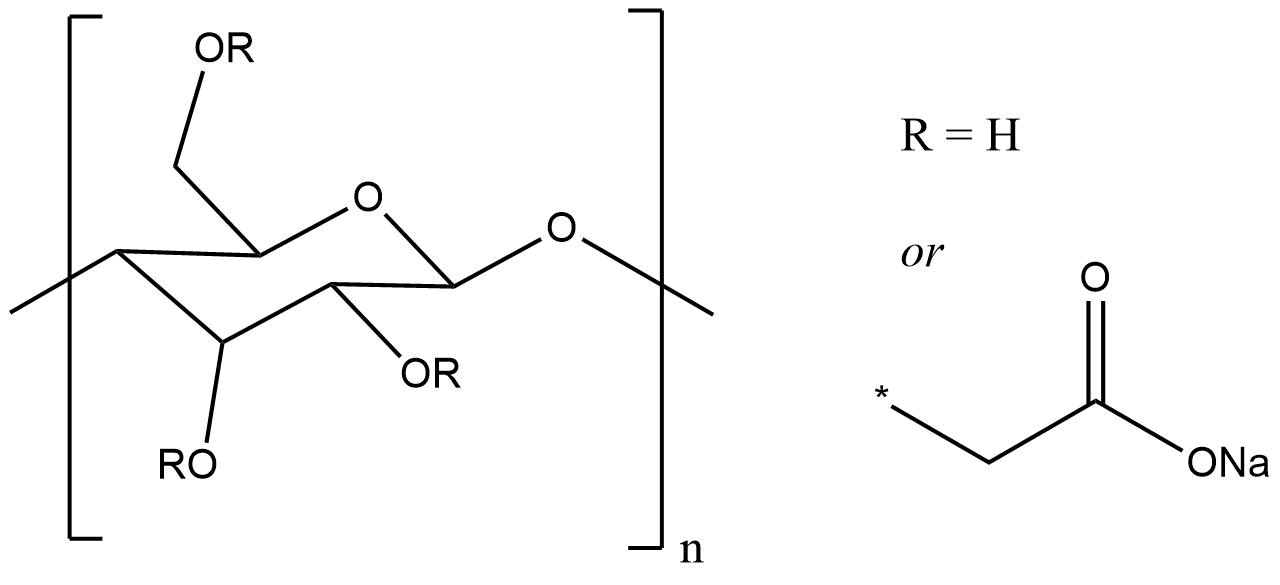
\includegraphics[width=0.8\columnwidth]{4-impregnation/figs/nc_structure.png}
    \caption{Structure of sodium carboxymethyl cellulose. Degree of substitution (DS) is taken as the average number of sodium carboxymethyl groups (\ce{-CH2COONa}) per monomer.}
    \label{fig:nc_structure}
\end{figure}

\section{Results \& Discussion}
\subsection{\texorpdfstring{Hydrothermal Sawdust \ce{KOH}-impregnation}{Hydrothermal Sawdust KOH-impregnation}}

\subsubsection{Porosity}

It was initially attempted to produce porous carbons via hydrothermal carbonisation with a KOH solution, i.e. without pyrolysis. Unsurprisingly this proved ineffective as activation typically requires temperatures in excess of 400 $^{\circ}C$. $A_{BET}$ of these samples (i.e. SH\textit{x.xx-TTT}) was not in excess of 10 $\rm m^2\ g^{-1}$.

\begin{table}[h]
    \caption{Porosity of SA\textit{x.xx-TTT} carbons}
    \label{tb:nc_porosity}
    \begin{tabularx}{\textwidth}{lllXXll}
    \toprule
        \textbf{Sample} & \multicolumn{2}{l}{$\mathbf{A_{BET}\ /\ m^2\ g^{-1}}$}  & \multicolumn{2}{l}{\textbf{Pore volume} / $\mathbf{cm^3\ g^{-1}}$} & \multicolumn{2}{l}{\textbf{Pore size / \AA}} \\
    \midrule
        \textbf{SA0.00-200} & & & & & \\
        \textbf{SA0.50-200} & & & & & \\
        \textbf{SA1.00-200} & & & & & \\
        \\
        \textbf{SA0.00-250} & 456 & (351) & 0.25 & (0.13) & \\
        \textbf{SA0.25-250} & & & & & \\
        \textbf{SA0.50-250} & 909 & (833) & 0.37 & (0.32) & \\
        \textbf{SA1.00-250} & 1081 & (973) & 0.45 & (0.37) & \\
        \textbf{SA2.00-250} & & & & & \\
        \\
        \textbf{SA0.00-300} & 326 & (247) & 0.17 & (0.10) & \\
        \textbf{SA0.50-300} & 1084 & (989) & 0.44 & (0.38) & \\
        \textbf{SA1.00-300} & 1295 & (1140) & 0.54 & (0.44) & \\
    \bottomrule
    \end{tabularx}
\end{table}

\paragraph{Density}

\subsection{Sodium Carboxymethyl Cellulose}

\subsubsection{Porosity}

\begin{table}[h]
    \caption{Porosity of NC\textit{x.x-TTT} carbons}
    \label{tb:nc_porosity}
    \begin{tabularx}{\textwidth}{llllXll}
    \toprule
        \textbf{Sample} & \multicolumn{2}{l}{$\mathbf{A_{BET}\ /\ m^2\ g^{-1}}$}  & \multicolumn{2}{l}{\textbf{Pore volume} / $\mathbf{cm^3\ g^{-1}}$} & \multicolumn{2}{l}{\textbf{Pore size / \AA}} \\
    \midrule
        \textbf{NC0.0-600} & 587 & (530) & 0.24 & (0.21) & \\
        \textbf{NC0.7-600} & 21 & (13) & 0.01 & (-) & \\
        \textbf{NC0.9-600} & 577 & (505) & 0.25 & (0.19) & \\
        \textbf{NC1.2-600} & 238 & (213) & 0.10 & (0.08) & \\
        \\
        \textbf{NC0.0-700} & 531 & (485) & 0.21 & (0.19) & \\
        \textbf{NC0.7-700} & 162 & (151) & 0.07 & (0.06) & \\
        \textbf{NC0.9-700} & 364 & (325) & 0.16 & (0.13) & \\
        \textbf{NC1.2-700} & 190 & (169) & 0.08 & (0.06) & \\
        \\
        \textbf{NC0.0-800} & 403 & (356) & 0.17 & (0.13) & \\
        \textbf{NC0.7-800} & 491 & (427) & 0.21 & (0.16) & \\
        \textbf{NC0.9-800} & 650 & (570) & 0.28 & (0.22) & \\
        \textbf{NC1.2-800} & 476 & (382) & 0.21 & (0.15) & \\
    \bottomrule
    \end{tabularx}
\end{table}

\section{Conclusion}

\bibliographystyle{rsc}
\bibliography{bibliography/bib}

\section*{Appendix}